% Koma class
\documentclass[a4paper, oneside]{scrartcl}   

\usepackage{a4wide}

%------------------
% language = english
\usepackage[english, german]{babel}	% Umlaute mit \"u
\usepackage[latin1]{inputenc}
\usepackage{enumitem}

% margins + Kopf- und Fusszeilen
\usepackage[left = 2.5cm, right = 2.5cm, top = 2cm, bottom = 3cm]{geometry}
\usepackage{scrpage2} 
\pagestyle{scrheadings}
\clearscrheadfoot
\rehead{\headmark}
\lehead{\pagemark}
\lohead{\headmark}
\rohead{\pagemark} 

% math
\usepackage{amssymb}
\usepackage{amsmath}

% figures
\usepackage{tikz}
\usepackage{graphicx}

% section-Zaehler wird neu gesetzt:
\setcounter{section}{10}
%------------------
\author{Sascha Meiers, Martin Seeger}
\title{Exercise 10, Discrete Mathematics for Bioinformatics}
\date{Winter term 2011/2012}


\begin{document}
\maketitle

%---------------------------------------------------------------------------------------------------

\subsection{Critical Mixed Cycles}

To be shown:
\[
T \subseteq E \textrm{ trace} \Longleftrightarrow \nexists \textrm{ critical
mixed cycle in } G' = (V, T, H)
\]

$\Rightarrow$: If $T$ is a trace then it corresponds to an alignment. In this
alignment, all edges in $T$ connect vertices in the same column and all arcs in
$H$ connect adjacent vertices in the same row in ascending order. Hence, along
an edge, the position index of the alignment stays always constant and along an
arc the position index of the alignment always increases. The cycle can
therefore never be closed.

$\Leftarrow$: Let us assume that $G'$ contains a mixed cycle $Z$ which is not
critical. Pick the smallest such cycle. By definition, there is one row $a^p$ in
the extended alignment graph for which $Z \cap a^p$ is non-consecutive. Call
$a^p_{i_0}$ the element in this row with highest position. Now cycle through $Z$
until you return to $Z \cap a^p$. 
If the return position is $a^p_{i_0}$ then
(because there must be other $a^p_i \in $ $Z \cap a^p$) we found a subcycle of $Z$ which
contradicts the choice of $Z$ as the smallest subcycle.
If the return position is $a^p_{i_1} \neq a^p_{i_0}$ then construct a cycle $Z' =
[a^p_{i_0} \ldots a^p_{i_1}] \cup [a^p_{i_1} \ldots a^p_{i_0}]$ where the second
component consists only of directed edges on $a^p$. Also $Z'$ is smaller than
$Z$, leading to a contradiction.
Therefore any mixed cycle in $G'$ must be critical. Inversely, no critical mixed
cycle means no cycle at all. 

Let us assume this is the case and construct an
alignment. We now consider the connected components $\{T_1,\ldots,T_n\}$ of
$(V, T)$. Let us connect $T_i$ and $T_j$ if any two of their elements are
connected in $H$. The resulting object is acyclic as it inherits the
acyclicality from $G'$. Hence we can topologically order it and thus induce a
strict partial order. This, according to the theorem by John Kececioglu, is
equvalent to $T$ realizing an alignment.$\square$

\subsection{Branch and Cut}

\renewcommand{\labelenumi}{\alph{enumi})}
\begin{enumerate}
  \item 
  Here you see the alignment graph $G=(V,E,H)$ (with only the 1-weighted edges drawn), 
  the conflict graph and the pair graph $PG(K_{p,q})$ for the two sequences $P$ and $Q$.
  
  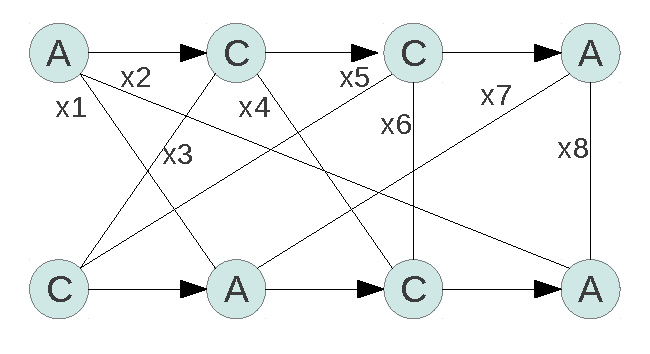
\includegraphics[width=6cm]{ex9_align_graph.pdf}
  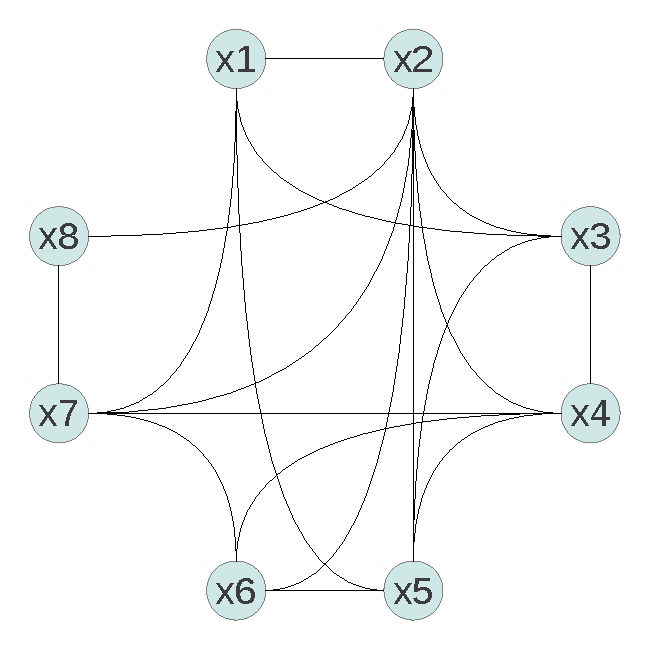
\includegraphics[width=4cm]{ex9_conflict_graph.pdf}
  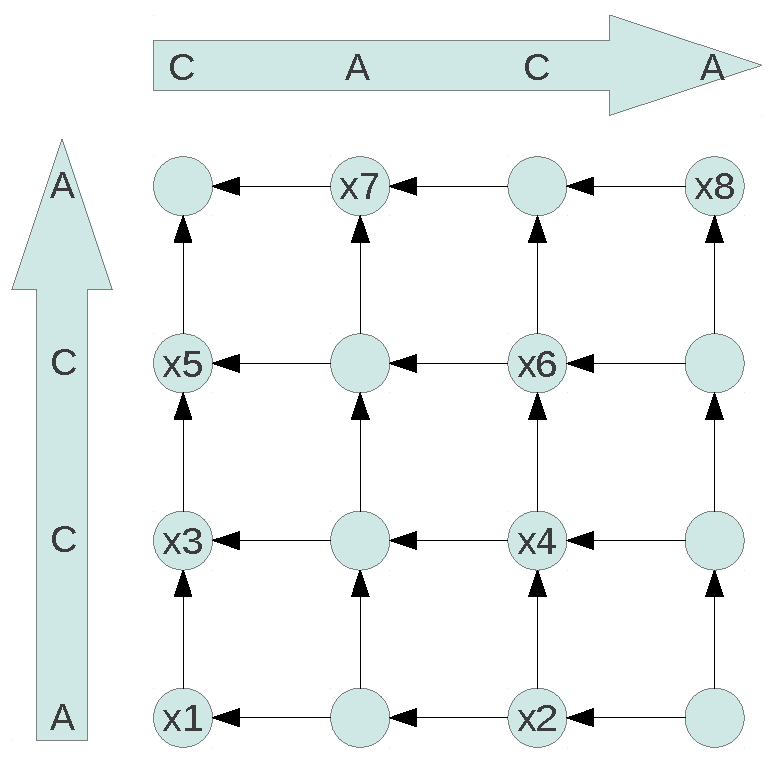
\includegraphics[width=4cm]{ex9_pair_graph.pdf}

  \item
  We start solving the LP relaxation of the problem without mixed cycle constraints:
  \begin{verbatim}
MAX x1 + x2 + x3 + x4 + x5  +x6 + x7 + x8

SUBJECT TO
A1:    - x1                                    <= 0
A2:         - x2                               <= 0
A3:              - x3                          <= 0
A4:                   - x4                     <= 0
A5:                        - x5                <= 0
A6:                             - x6           <= 0
A7:                                  - x7      <= 0
A8:                                       - x8 <= 0
B1:    + x1                                    <= 1
B2:         + x2                               <= 1
B3:              + x3                          <= 1
B4:                   + x4                     <= 1
B5:                        + x5                <= 1
B6:                             + x6           <= 1
B7:                                  + x7      <= 1
B8:                                       + x8 <= 1  
  \end{verbatim}
  \begin{enumerate}
    \item optimal value $8$, $(1,1,1,1,1,1,1,1)$ \\ 
          heaviest source-to-sink path: $4 > 1$ \\
          Adding inequality \texttt{x2 + x4 + x6 + x7 <= 1}
    \item optimal value $5$, $(1,0,1,0,1,0,1,1)$ \\ 
          heaviest source-to-sink path: $3 > 1$ \\
          Adding inequality \texttt{x1 + x2 + x3 + x5 <= 1}
    \item optimal value $3$, $(1,0,0,0,0,0,1,1)$ \\ 
          heaviest source-to-sink path: $2 > 1$ \\
          Adding inequality \texttt{x7 + x8 <= 1}
    \item optimal value $3$, $(1,0,0,0,0,1,0,1)$ \\ 
          heaviest source-to-sink path: $1 \leq 1$ \\
          integral solution $\Rightarrow$ done
  \end{enumerate}
\end{enumerate}

\subsection{Branch and Cut}

\renewcommand{\labelenumi}{\alph{enumi})}
\begin{enumerate}
  \item Again we start solving the LP relaxation of the problem without mixed cycle constraints:
  
  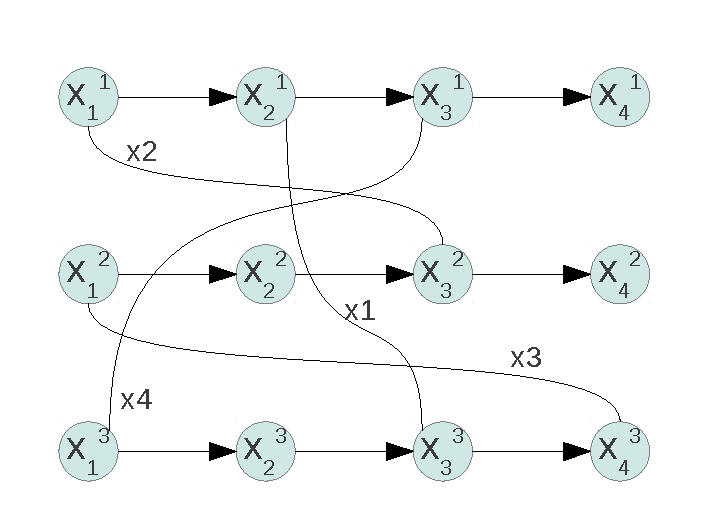
\includegraphics[width=6cm]{ex9_align_graph_task3.pdf}
  
  \begin{verbatim}
MAX x1 + x2 + x3 + x4

SUBJECT TO
A1:    - x1                <= 0
A2:         - x2           <= 0
A3:              - x3      <= 0
A4:                   - x4 <= 0
B1:    + x1                <= 1
B2:         + x2           <= 1
B3:              + x3      <= 1
B4:                   + x4 <= 1
  \end{verbatim}
  \begin{enumerate}
    \item optimal value $4$, $(1,1,1,1)$ \\ 
          shortest path from any node $x_i$ to $x_{i-1}$: $(x_2^3, x_1^3)$ with length 0 \\
          Adding inequality \texttt{x1 + x4 <= 1}
    \item optimal value $3$, $(1,1,1,0)$ \\ 
          shortest path from any node $x_i$ to $x_{i-1}$: $(x_4^3, x_3^3)$ with length 0 \\
          Adding inequality \texttt{x1 + x2 + x3 <= 2}
    \item optimal value $3$, $(0,1,1,1)$ \\ 
          shortest path from any node $x_i$ to $x_{i-1}$: $(x_4^3, x_3^3)$ with length 0 \\
          Adding inequality \texttt{x2 + x3 + x4 <= 2}
    \item optimal value $2.5$, $(0.5,1,0.5,0.5)$ \\ 
          shortest path from any node $x_i$ to $x_{i-1}$: $(x_3^3, x_2^3)$ with length 1 \\
          Could not find a solution!
  \end{enumerate}
  
  \item \textbf{Branching}\\
        It is not difficult to find a feasible solution with value $2$, choosing $x_2$ and $x_3$
        (\emph{global lower bound}). The current \emph{local upper bound} is $2.5$.
        
        First branch: $x1 = 0 \Rightarrow$ optimal value $2$, solution $(0,1,0,1) \Rightarrow$ done!
        
        (need no further branch)
  
  \item Adding the constraint \texttt{x1 + x2 + x3 + x4 <= 2} to the inequalities from part (a) 
        directly leads to a solution with optimal value $2$ and chosen edges $x_1$ and $x_2$
  
  \item Proof:


\end{enumerate}

\end{document}
